\documentclass{article}

\usepackage[english]{babel}

\usepackage{float}

\usepackage{paralist}

\usepackage{graphicx}

\usepackage[tight,footnotesize]{subfigure}

 \graphicspath{  {/Users/Luis/Documents/GW/MAE6225_cfd/ccg_poisson/latex_plots/} }

\DeclareGraphicsExtensions{.png,.pdf, .jpg}

\usepackage[a4paper, inner=1.5cm, outer=3cm, top=2cm, bottom=3cm, bindingoffset=1cm]{geometry}

\usepackage{amsmath}

\begin{document}

\pagestyle{plain}

\title{MAE 6225 Project 1: Solving the 2-D Poisson Equation with Jacobi and Successive Over-Relaxation Methods}
\author{Luis Martinez}
\date{March 16, 2016}
\maketitle
%%%%%%%%%%%%%%%%%%%%%%

\section{Introduction}


\noindent This paper presents solutions to two test cases of the 2-D Poisson Equation using different iterative solvers. The iterative solvers studied are the Jacobi, Gauss-Sidel, and Successive Over-Relaxation (SOR) techniques. The Poisson equation was discretized using a second-order central finite difference scheme. The grid employed is a cell-centered node approach (see figure 1).

\vspace{1em}

\noindent The test cases observed correspond to different source term functions. These are:\\

\indent  - Case 1: Homogeneous Dirichlet boundary conditions, and $f(x,y) = -8 sin(2 \pi n x ) sin(2 \pi n y )$\\
\indent  - Case 2: Homogeneous Neumann boundary conditions, and $f(x,y) = -8 cos(2 \pi n x ) cos(2 \pi n y)$\\

\noindent In these cases, $n$ represents frequency. We examine solutions for different frequencies and how solution parameters need to be modified based on these frequencies. Section 2 provides details of the derivation of the numerical scheme; Section 3 contains a discussion of boundary conditions, Section 4 provides results for the $1^{st}$ case; and $2^{nd}$ case; and Section 5 summarizes how the SOR solution is affected by the relaxation parameter $\omega$ , frequency, number of grid points, and boundary conditions.

%%%%%%%%%%%%%%%%%%%%%%
\section{Discretization of the Poisson Equation \\ and Iterative Methods}

\noindent The 2-D Poisson equation is discretized using a second-order finite difference scheme consistent with the cell-centered grid system for computation. We begin the process of discretization by stating the 2-D equation, which looks like this:

\begin{equation}
f(x,y) = \frac{\partial^2 \phi (x,y)}{\partial x^2} +  \frac{\partial^2 \phi (x,y)}{\partial y^2} 
\end{equation}

\noindent Now, using a second-order approximation, we can express the equation as such:

\begin{equation}
f_{i,j} = \frac{ \phi_{i+1,j}  - 2 \phi_{i,j} + \phi_{i-1,j} }{\Delta x^2} + \frac{\phi_{i,j+1}  - 2 \phi_{i,j} + \phi_{i,j-1}}{\Delta y^2}
\end{equation}

\noindent The  objective here is to find an expression for the unknown variable $\phi_{i,j} $, and with some algebraic manipulations we can find this expression.

\begin{align}
f_{i,j} &= \frac{  \bigg(  \phi_{i+1,j}   + \phi_{i-1,j}  \bigg)\Delta y^{2} +  \bigg( \phi_{i,j+1}  + \phi_{i,j-1}  \bigg)\Delta x^{2}   }{\Delta x^{2} \Delta y^{2}}  - \frac{2 \phi_{i,j} \bigg( \Delta x^{2} +  \Delta y^{2} \bigg) }{\Delta x^{2} \Delta y^{2}} \nonumber \\
\phi_{i,j} &=  \frac{  \bigg(  \phi_{i+1,j}   + \phi_{i-1,j}  \bigg)\Delta y^{2} +  \bigg( \phi_{i,j+1}  + \phi_{i,j-1}  \bigg)\Delta x^{2}   }{ 2 ( \Delta x^{2} + \Delta y^{2} )} - \frac{\Delta x^{2} \Delta y^{2} f_{i,j}}{2 ( \Delta x^{2} + \Delta y^{2} )}
\end{align}

\vspace{1em}

\noindent Equation (3) above is the discretized form that we will use and modify to solve using the different iterative techniques. Let's observe how the different methods approach the solution.

%%%
\subsection{Jacobi method}
%%%

\noindent With the Jacobi method as with all other methods considered in this paper, we initialize the field with an initial guess. This initial guess is then used to initiate the iterative process and find the computed solution at the next iterative cylce. Then, equation (3) can be modified to obtain the  solution at the next cycle:

\begin{equation}
\phi_{i,j}^{k+1} =  \frac{  \bigg(  \phi_{i+1,j}^{k}   + \phi_{i-1,j}^{k}  \bigg)\Delta y^{2} +  \bigg( \phi_{i,j+1}^{k}  + \phi_{i,j-1}^{k}  \bigg)\Delta x^{2}   }{ 2 ( \Delta x^{2} + \Delta y^{2} )} - \frac{\Delta x^{2} \Delta y^{2} f_{i,j}}{2 ( \Delta x^{2} + \Delta y^{2} )}
\end{equation}

\vspace{1em}

\noindent Note that in equation (4) the subscript $k$ corresponds to the solution at the previous iteration cycle and $k+1$ represents the solution at the current cycle. 

%%%
\subsection{Gauss-Sidel Method}
%%%

\noindent The Gauss-Sidel (GS) method improves the Jacobi method by using updated values as soon as they are obtained. Figure 1 shows the sweep direction for the GS method used in this paper. Using the sweep direction shown in this figure, we can modify the Jacobi method, and the new solution is expressed as:

\begin{equation}
\phi_{i,j}^{k+1} =  \frac{  \bigg(  \phi_{i+1,j}^{k}   + \phi_{i-1,j}^{k+1}  \bigg)\Delta y^{2} +  \bigg( \phi_{i,j+1}^{k}  + \phi_{i,j-1}^{k+1}  \bigg)\Delta x^{2}   }{ 2 ( \Delta x^{2} + \Delta y^{2} )} - \frac{\Delta x^{2} \Delta y^{2} f_{i,j}}{2 ( \Delta x^{2} + \Delta y^{2} )}
\end{equation}


%%%%%%%%%%%%%%%%%%%%%%%%%%%%%%%%%%%%%%%
\begin{figure}[H]
\centering
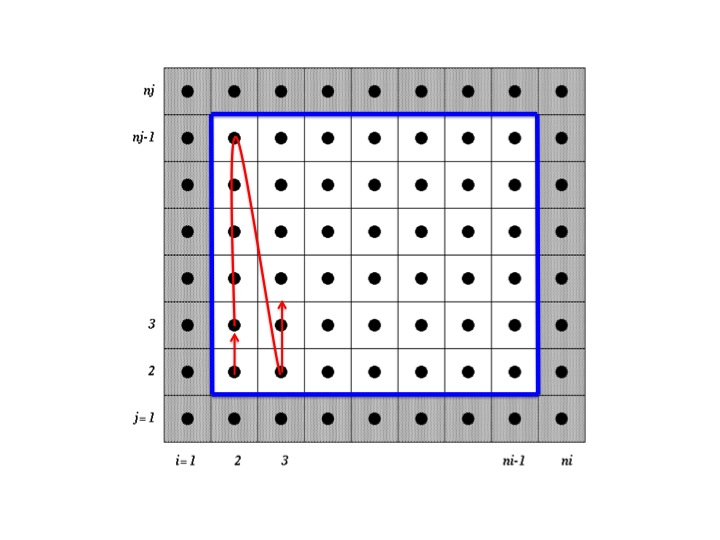
\includegraphics[width=0.7\textwidth]{grid}\label{Grid}
\caption{Direction (red arrow) of Gauss-Sidel sweep in the algorithm. The shaded region represents ghost cells, while the blue represents the boundary. }
\end{figure}
%%%%%%%%%%%%%%%%%%%%%%%%%%%%%%%%%%%%%%%%%%

\newpage

%%%%%%%%%%%%%%%%%%%%%%%%%%%%%%%%%%%%%%%%%%%

\subsection{Successive Over-Relaxation (SOR) Method}

Yet another approach to solve these cases is to use the SOR method. In this case, a relaxation parameter $ ( \omega )$ is introduced to improve on the guesses determined by the Gauss-Sidel method. The SOR method can be expressed as:

\begin{equation}
\phi_{i,j}^{k+1} =  (1 - \omega ) \phi_{i,j}^{k}  +  \omega \frac{  \bigg(  \phi_{i+1,j}^{k}   + \phi_{i-1,j}^{k+1}  \bigg)\Delta y^{2} +  \bigg( \phi_{i,j+1}^{k}  + \phi_{i,j-1}^{k+1}  \bigg)\Delta x^{2}   }{ 2 ( \Delta x^{2} + \Delta y^{2} )} - \omega \frac{\Delta x^{2} \Delta y^{2} f_{i,j}}{2 ( \Delta x^{2} + \Delta y^{2} )}
\end{equation}

\vspace{1em}

\noindent Note that equation (6) tells us that when $\omega =1$, we return to the Gauss-Sidel method. When $\omega < 1$, the solution is "under-relaxed", and when $\omega > 1$, the solution is over-relaxed. As we will see below, we have to be careful when choosing these relaxation parameters.

%%%%%%%%%%%%%%%%%%%%%%%%%%%%%%%%%%%%%%%%%%%
\section{Boundary Conditions}
 
\noindent For case 1, the boundary conditions would be straightforward if we were using nodes on the boundary. However, because we have the cell-centered system, we need to make sure we derive the proper equations. Similarly, for case 2, we also need to derive the proper equations at the edge nodes. Let's look at case 1 first.

\vspace{1em}

\noindent Using the lower edge nodes as shown by figure (1), we can derive the adequate Poisson equation at these nodes. Figure (2) shows the stencil used for the lower edge nodes.

%%%%%%%%%%%%%%%%%%%%%%%%%%%%%%%%%%%%%%%
\begin{figure}[H]
\centering
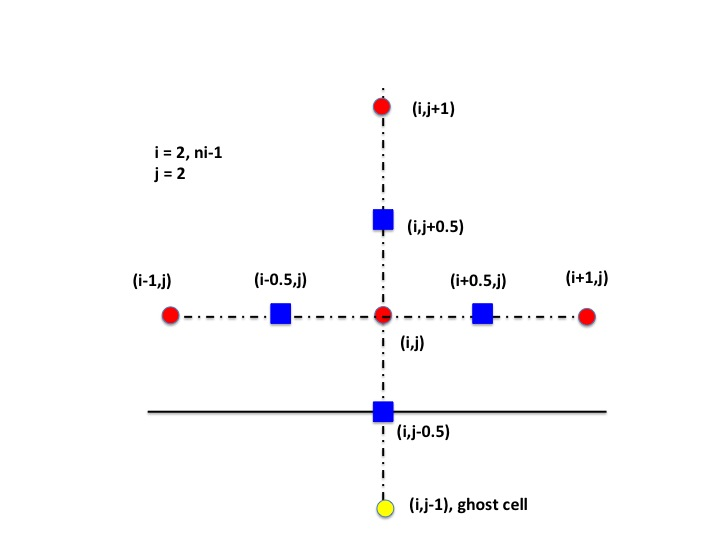
\includegraphics[width=0.7\textwidth]{stencil_bc}\label{stencil}
\caption{Nodes used to derive expressions for $\phi_{i,j} $ at the lower edge nodes. A similar process is performed for the other three boundaries and four corners. }
\end{figure}
%%%%%%%%%%%%%%%%%%%%%%%%%%%%%%%%%%%%%%%%%%

\vspace{1em}
\newpage

\subsection{Case 1 - Homogeneous Dirichlet Boundaries}

\vspace{1em}

\noindent Using figure (2), for case 1 we can express the second derivatives  at these edge nodes as follows:

\begin{align}
\frac{\partial^2 \phi (i,j)}{\partial y^2}  &=  \frac{1}{{y_{i, j+0.5} - y_{i, j-0.5}}}  \bigg( \frac{\partial \phi_{i, j+0.5}}{\partial y} - \frac{\partial \phi_{i, j-0.5}}{\partial y} \bigg)    \nonumber   \\
\frac{\partial^2 \phi (i,j)}{\partial y^2}  &= \frac{1}{{y_{i, j+0.5} - y_{i, j-0.5}}}  \bigg(  \frac{ \phi_{i,j+1} - \phi_{i,j} }{y_{i,j+1} - y_{i,j}}  -  \frac{ \phi_{i,j} - \phi_{i,j-0.5} }{y_{i,j} - y_{i,j-0.5}}   \bigg) \nonumber  \vspace{1 em}  \\
\frac{\partial^2 \phi (i,j)}{\partial y^2}  &= \frac{1}{\Delta y}  \bigg(  \frac{ \phi_{i,j+1} - \phi_{i,j} }{\Delta y}  -  \frac{ \phi_{i,j} - \phi_{i,j-0.5} }{0.5 \Delta y}   \bigg) \nonumber \vspace{1 em}  \\
\frac{\partial^2 \phi (i,j)}{\partial y^2}  &= \frac{  \phi_{i,j+1} - 3 \phi_{i,j} + 2 \phi_{i,j-0.5} }{\Delta y^{2}} \nonumber
\end{align}

\vspace{1em}

\noindent We know that for case 1, $\phi_{i,j-0.5} $ is zero because of the specified homogeneous dirichlet conditions, so we can simplify our expression to:

\begin{align}
\frac{\partial^2 \phi (i,j)}{\partial y^2}  &= \frac{  \phi_{i,j+1} - 3 \phi_{i,j}  }{\Delta y^{2}} \nonumber
\end{align}

\vspace{1em}

\noindent For the x second derivative, we can simply use the neighboring cell-center nodes to obtain:

\begin{align}
\frac{\partial^2 \phi (i,j)}{\partial x^2}  &= \frac{  \phi_{i+1,j} - 2 \phi_{i,j} +  \phi_{i-1,j} }{\Delta y^{2}} \nonumber
\end{align}

\vspace{1em}

\noindent Then, combining the derivatives and solving for $\phi_{i,j}$ :

\begin{equation}
\phi_{i,j} = \frac{ \Delta x^{2} \big(  \phi_{i,j+1} \big) + \Delta y^2 \big(  \phi_{i+1,j} + \phi_{i-1,j} \big) - \Delta x^{2} \Delta y^{2} f_{i,j}}{3 \Delta x^2  + 2 \Delta y^2} \ \ \ i=2,ni-1, \ \ \ j=2 
\end{equation}

\vspace{1em}

\noindent Repeating this process for all boundaries and corners, we can complete the equations at the boundaries for case 1:

\begin{align}
\phi_{i,j} &= \frac{ \Delta x^{2} \big(  \phi_{i,j-1}  \big) + \Delta y^2 \big(  \phi_{i+1,j} + \phi_{i-1,j} \big) - \Delta x^{2} \Delta y^{2} f_{i,j} }{3 \Delta x^2  + 2 \Delta y^2} \ \ \ i=2,ni-1, \ \ \ j=nj-1 \\
\phi_{i,j} &= \frac{ \Delta x^{2} \big( \phi_{i,j+1} + \phi_{i,j-1}  \big) + \Delta y^2 \big(  \phi_{i+1,j}  \big) - \Delta x^{2} \Delta y^{2} f_{i,j} }{3 \Delta y^2  + 2 \Delta x^2} \ \ \ j=2,nj-1, \ \ \ i=2 \\
\phi_{i,j} &= \frac{ \Delta x^{2} \big( \phi_{i,j+1} + \phi_{i,j-1}  \big) + \Delta y^2 \big(  \phi_{i-1,j}  \big) - \Delta x^{2} \Delta y^{2} f_{i,j} }{3 \Delta y^2  + 2 \Delta x^2} \ \ \ j=2,nj-1, \ \ \ i=ni-1 \\
\phi_{i,j} &= \frac{ \Delta x^{2} \big( \phi_{i,j-1}  \big) + \Delta y^2 \big(  \phi_{i+1,j}  \big) - \Delta x^{2} \Delta y^{2} f_{i,j} }{3 \Delta y^2  + 3 \Delta x^2} \ \ \ i=2 \ \ \ j=nj-1 \\
\phi_{i,j} &= \frac{ \Delta x^{2} \big( \phi_{i,j+1}  \big) + \Delta y^2 \big(  \phi_{i+1,j}  \big) - \Delta x^{2} \Delta y^{2} f_{i,j} }{3 \Delta y^2  + 3 \Delta x^2} \ \ \ i=2 \ \ \ j=2 \\
\phi_{i,j} &= \frac{ \Delta x^{2} \big( \phi_{i,j-1}  \big) + \Delta y^2 \big(  \phi_{i-1,j}  \big) - \Delta x^{2} \Delta y^{2} f_{i,j} }{3 \Delta y^2  + 3 \Delta x^2} \ \ \ i=ni-1 \ \ \ j=nj-1 \\
\phi_{i,j} &= \frac{ \Delta x^{2} \big( \phi_{i,j+1}  \big) + \Delta y^2 \big(  \phi_{i-1,j}  \big) - \Delta x^{2} \Delta y^{2} f_{i,j} }{3 \Delta y^2  + 3 \Delta x^2} \ \ \ i=ni-1 \ \ \ j=2 
\end{align}

\vspace{1em}

\noindent Equations (7) through (14) are the complete set of equations for the boundary conditions at the edge cell-centered nodes. Now let's look at case 2.

\subsection{Case 2 - Homogeneous Neumann Boundaries}

\vspace{1em}

\noindent Following a similar process as described for case 1, the objective is to approximate the second derivatives with values we can use in the flow-field. In this case, a useful approximation is to state that the edge nodes are approximately equal to the ghost cells due to the imposed boundary condition. Then, using the lower boundary again as an example, we can say that $\phi_{i,j} \approx \phi_{i,j-1}$. Then, for case 2 we can express the complete set of boundary equations:

\begin{align}
\phi_{i,j} &= \frac{ \Delta x^{2} \big( \phi_{i,j+1}  \big) + \Delta y^2 \big(  \phi_{i+1,j} + \phi_{i-1,j} \big) - \Delta x^{2} \Delta y^{2} f_{i,j} }{2 \Delta y^2  +  \Delta x^2} \ \ \ i=2,ni-1 \ \ \ j=2 \\
\phi_{i,j} &= \frac{ \Delta x^{2} \big( \phi_{i,j-1}  \big) + \Delta y^2 \big(  \phi_{i+1,j} + \phi_{i-1,j} \big) - \Delta x^{2} \Delta y^{2} f_{i,j} }{2 \Delta y^2  +  \Delta x^2} \ \ \ i=2,ni-1 \ \ \ j=nj-1 \\
\phi_{i,j} &= \frac{ \Delta x^{2} \big( \phi_{i,j+1} +  \phi_{i,j-1}   \big) + \Delta y^2 \big( \phi_{i+1,j} \big) - \Delta x^{2} \Delta y^{2} f_{i,j} }{ \Delta y^2  +  2 \Delta x^2} \ \ \ i=2 \ \ \ j=2,nj-1 \\
\phi_{i,j} &= \frac{ \Delta x^{2} \big( \phi_{i,j+1} +  \phi_{i,j-1}   \big) + \Delta y^2 \big( \phi_{i-1,j} \big) - \Delta x^{2} \Delta y^{2} f_{i,j} }{ \Delta y^2  +  2 \Delta x^2} \ \ \ i=ni-1 \ \ \ j=2,nj-1 \\
\phi_{i,j} &= \frac{ \Delta x^{2} \big( \phi_{i,j+1}  \big) + \Delta y^2 \big(  \phi_{i+1,j}  \big) - \Delta x^{2} \Delta y^{2} f_{i,j} }{ \Delta y^2  +  \Delta x^2} \ \ \ i=2 \ \ \ j=2 \\
\phi_{i,j} &= \frac{ \Delta x^{2} \big( \phi_{i,j-1}  \big) + \Delta y^2 \big(  \phi_{i+1,j}  \big) - \Delta x^{2} \Delta y^{2} f_{i,j} }{ \Delta y^2  +  \Delta x^2} \ \ \ i=2 \ \ \ j=nj-1 \\
\phi_{i,j} &= \frac{ \Delta x^{2} \big( \phi_{i,j-1}  \big) + \Delta y^2 \big(  \phi_{i-1,j}  \big) - \Delta x^{2} \Delta y^{2} f_{i,j} }{ \Delta y^2  +  \Delta x^2} \ \ \ i=ni-1 \ \ \ j=nj-1 \\
\phi_{i,j} &= \frac{ \Delta x^{2} \big( \phi_{i,j+1}  \big) + \Delta y^2 \big(  \phi_{i-1,j}  \big) - \Delta x^{2} \Delta y^{2} f_{i,j} }{ \Delta y^2  +  \Delta x^2} \ \ \ i=ni-1 \ \ \ j=2 
\end{align}

\vspace{1em}

\noindent Equations (15) through (22) are the complete set of equations for the boundary conditions at the edge cell-centered nodes for case 2.

\section{Test Cases}

\noindent In this section we will loot at two different cases using different source terms and boundary conditions. We will perform iteration and grid convergence analysis for both cases.

\subsection{Case 1: Source Term with Homogeneous Dirichlet Boundary Conditions}

\noindent In this section we'll look at results obtained from the three different iterative methods, as well as convergence and grid refinements studies. We will also examine the effect of varying the source term frequency on our convergence and errors. To start, let's look at the simplest case: the solution for a frequency of $n = 1$. The solution is initiated by assigning random numbers from 0 to 1 in the entire flow field. This initial guess is then passed into the iterative solvers.

\vspace{1em}

\noindent Figure (3) shows how the analytical solution looks compared to the computed solutions on a 3-D topographical representation. Figure (3) visually show that the general shapes of the analytical and computed solutions $appear$ to be similar. If you look closely the computed solutions all appear to exceed analytical maximum and minimum (values of [1,-1] ). The maximum and minimum values for the different methods did not vary significantly for our analysis, and all were within 99.9 percent of the analytical minimum and maximum.

\newpage

\vspace{10em}

%%%%%%%%%%%%%%%%%%%%%%%%%%%%%%%%%%%%%%%
\begin{figure}[H]
\centering
\subfigure[]{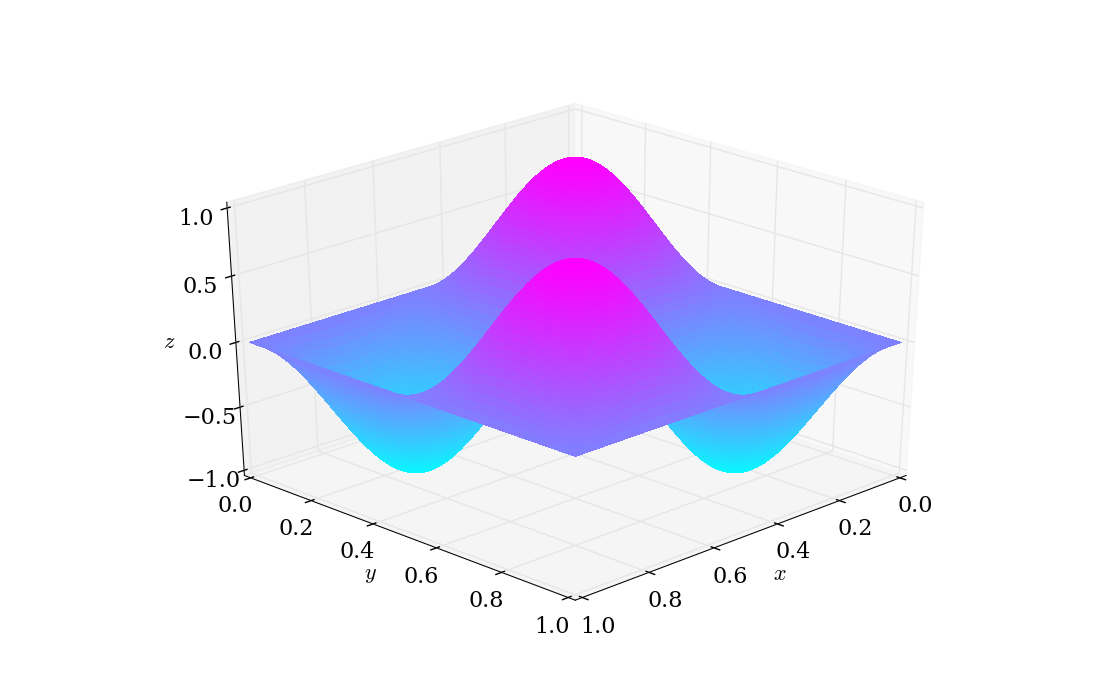
\includegraphics[width=0.4\textwidth]{p_an3d}\label{analytical function 3D}}
\subfigure[]{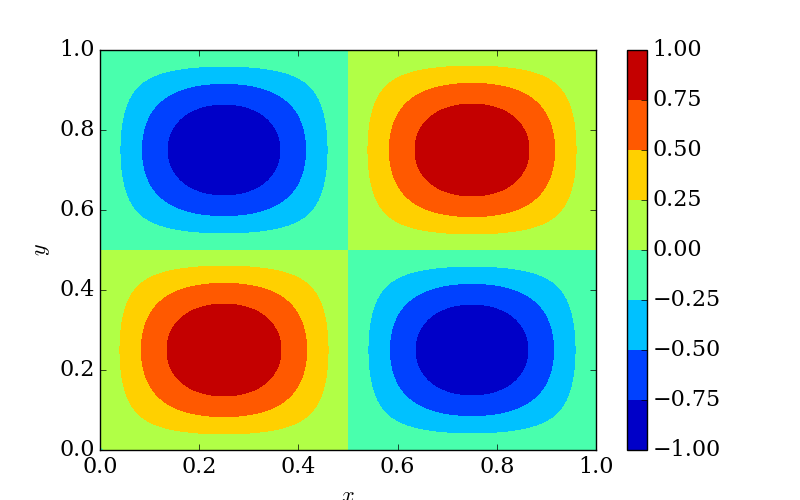
\includegraphics[width=0.4\textwidth]{p_an2d}\label{analytical function 2D}}
%\hspace{1em}
\subfigure[]{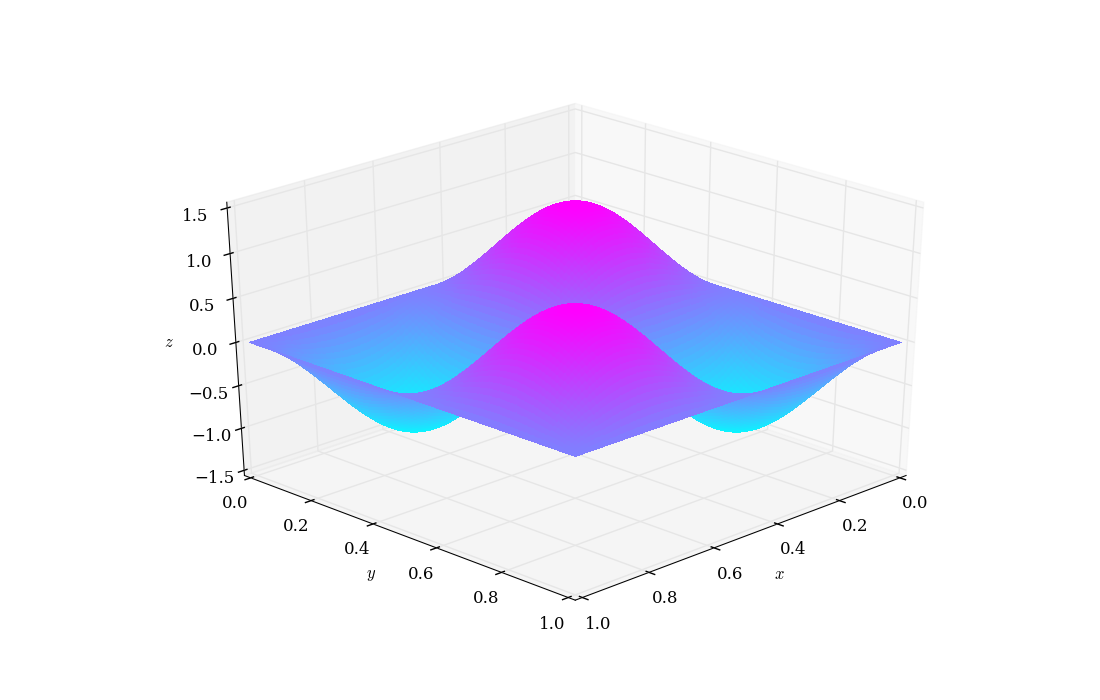
\includegraphics[width=0.4\textwidth]{J_3D_case1}\label{Jacobi 3D}}
\subfigure[]{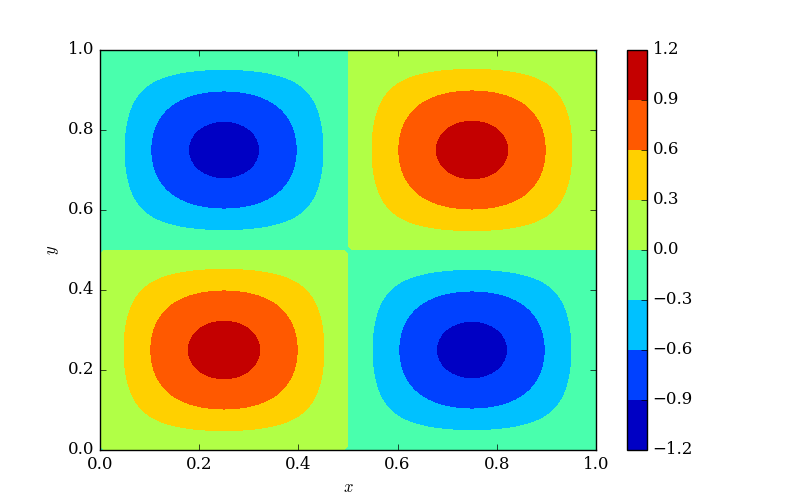
\includegraphics[width=0.4\textwidth]{J_2D_case1}\label{Jacobi 2D}}
%\hspace{1em}
\subfigure[]{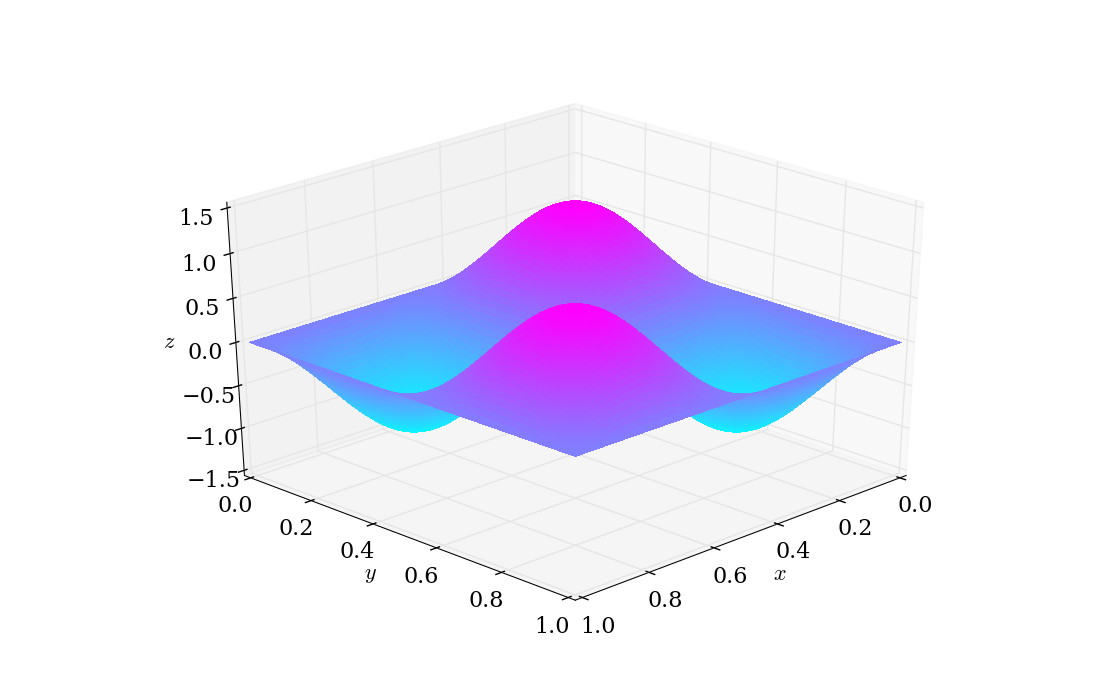
\includegraphics[width=0.4\textwidth]{pGS3d}\label{GS 3D}}
\subfigure[]{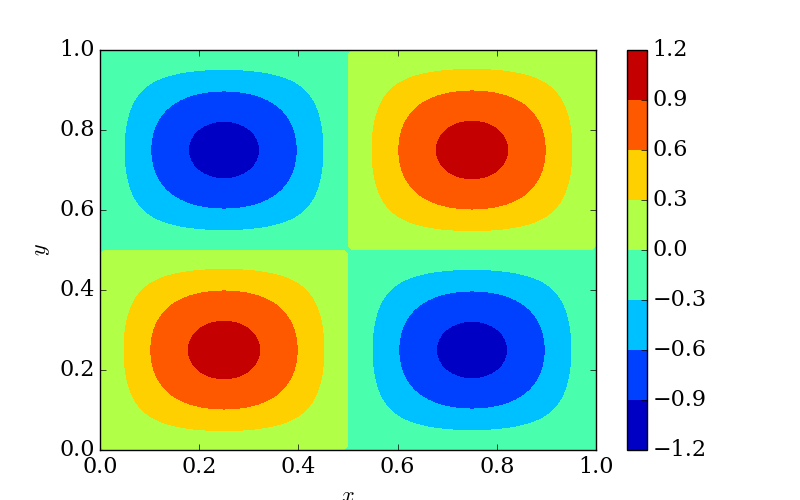
\includegraphics[width=0.4\textwidth]{pGS2d}\label{GS 2D}}
%\hspace{1em}
\subfigure[]{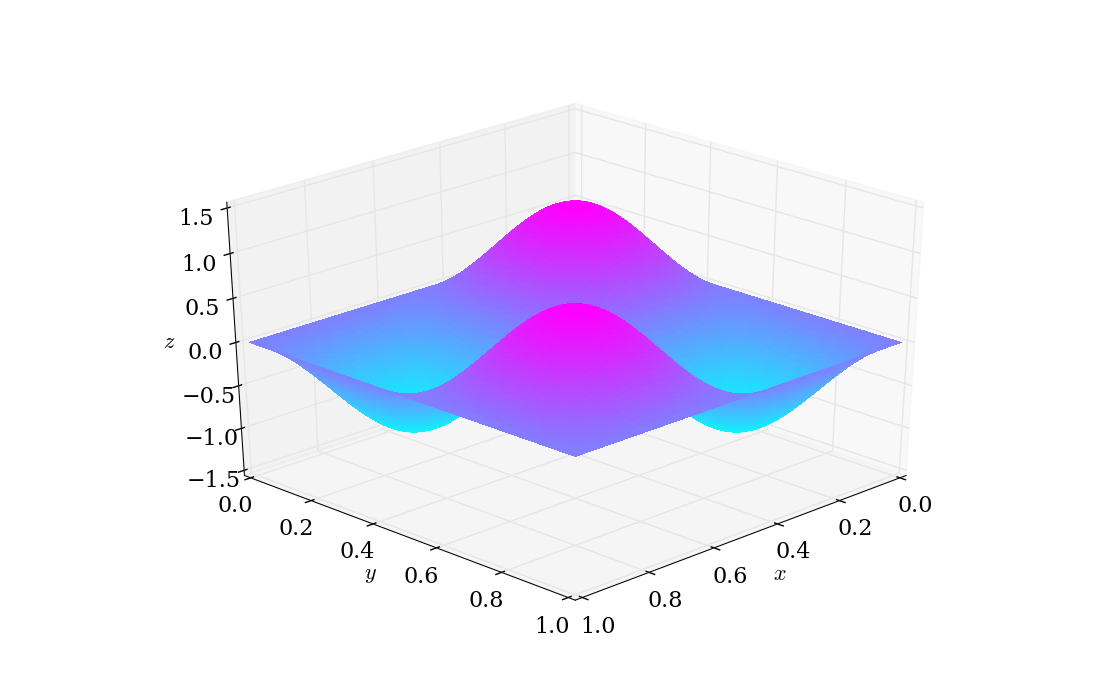
\includegraphics[width=0.4\textwidth]{pSOR3d}\label{SOR 3D}}
\subfigure[]{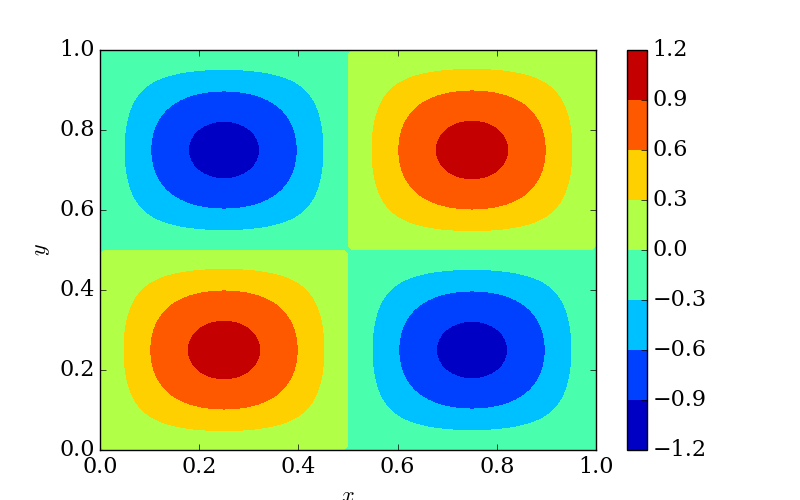
\includegraphics[width=0.4\textwidth]{pSOR2d}\label{SOR 2D}}
\caption{Visual comparison of analytical and computed solutions. (a-b) analytical solution, (b-c) Jacobi, (d-e) Gauss-Sidel, (f-g) SOR }
\end{figure}
%%%%%%%%%%%%%%%%%%%%%%%%%%%%%%%%%%%%%%%%%%

\newpage

\noindent Now, lets observe how these methods converged to the target error. Figure (4) shows the iterations required by each method to converge to the l2 norm of the error. We can clearly see the improvements made by the Gauss-Sidel method in comparison to the Jacobi method, and we can also see that the SOR ($\omega = 1.9 $) required less than one-fourth of the iterations needed by the Gauss-Sidel Method. We'll discuss the choice of relaxation parameter below.

%%%%%%%%%%%%%%%%%%%%%%%%%%%%%%%%%%%%%%%
\begin{figure}[H]
\centering
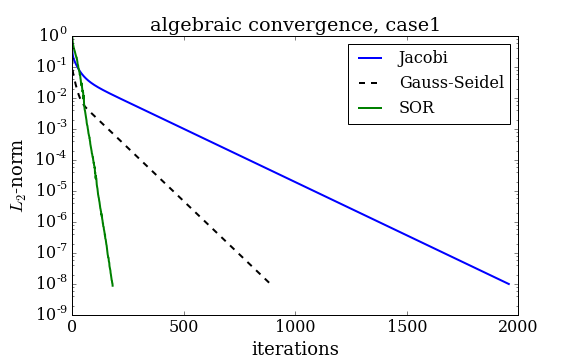
\includegraphics[width=0.7\textwidth]{algb_conv_c1_g1_w1}\label{Algebraic Convergence}
\caption{Convergence of the iterative methods for case 1 with a frequency of n=1. }
\end{figure}
%%%%%%%%%%%%%%%%%%%%%%%%%%%%%%%%%%%%%%%%%%

\vspace{1em}

\noindent Now we are poised to examine how these methods compared to the analytical solution by looking at the l2 norm of the error and by using different grid sizes. For this analysis, I chose an array of grid points with x and y grid points being the same. The array of grid points used for this analysis is described as:

\begin{equation}
n_{x} = n_{y} = [25, 50, 100, 150, 200] \nonumber
\end{equation}

\vspace{1em}

\noindent Figure (5) on the next page shows that the error looks like a second-order error, which is consistent with our discretization scheme. The error decreases as we refine the grid.

\vspace{1em}

\noindent At this point, we still need to understand what happens to the computed solution with increasing frequency. Also, we have to take a closer look at the impact of different relaxation parameters for the SOR method.

\vspace{1em}

\noindent Building on the simple case with $(n=1)$, we can look at how the SOR method converges based on different relaxation parameters. We can perform a convergence test to our solution with the following relaxation parameters:

\begin{equation}
\omega = [1.2,1.4,1.6,1.8,1.9] \nonumber
\end{equation}

\noindent Figure (6) shows convergence rates by increasing omega . It is also interesting to note that  the solution converges the fastest with $\omega = 1.8$.



%%%%%%%%%%%%%%%%%%%%%%%%%%%%%%%%%%%%%%%
\begin{figure}[H]
\centering
\subfigure[]{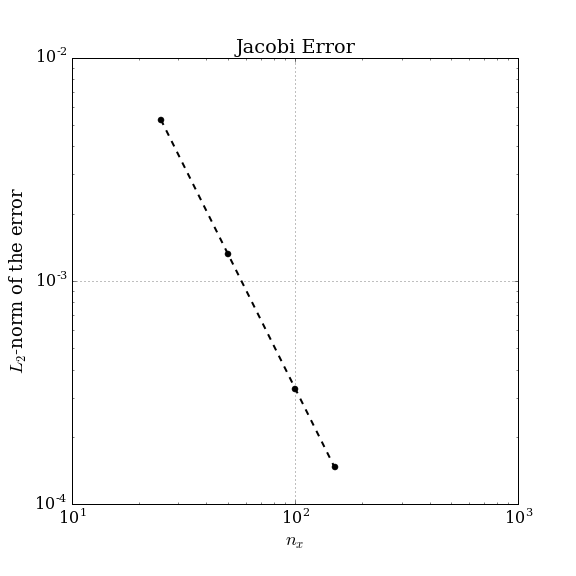
\includegraphics[width=0.5\textwidth]{errj_c1_g1_w1}\label{jacobi error 1}}
\subfigure[]{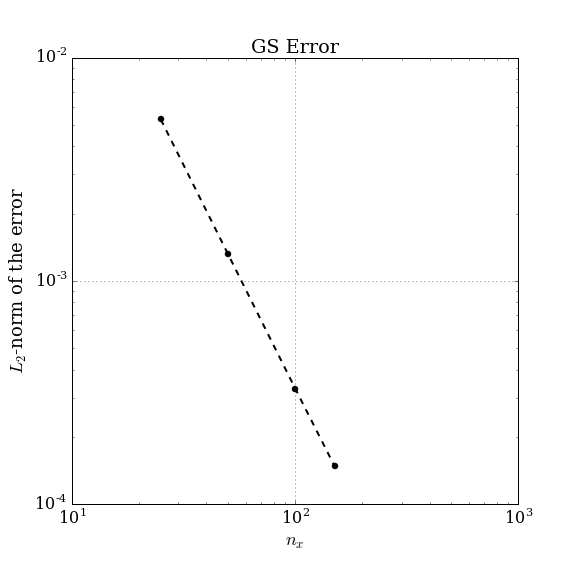
\includegraphics[width=0.5\textwidth]{errgs_c1_g1_w1}\label{gs error}}
\subfigure[]{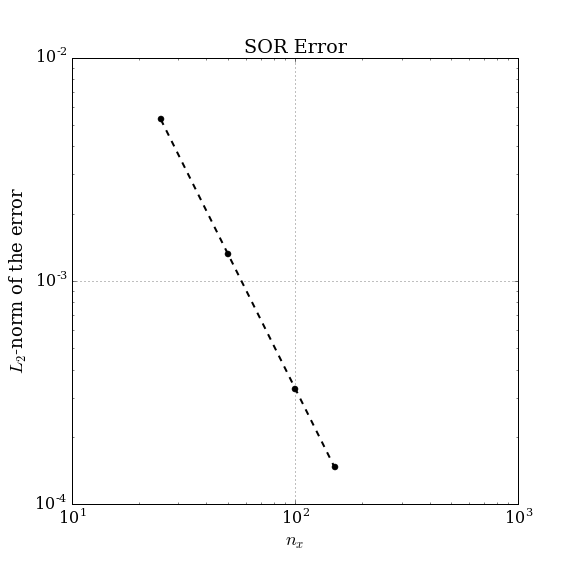
\includegraphics[width=0.5\textwidth]{errsor_c1_g1_w1}\label{sor error}}
\caption{Grid Refinement}
\end{figure}
%%%%%%%%%%%%%%%%%%%%%%%%%%%%%%%%%%%%%%%%%%

%%%%%%%%%%%%%%%%%%%%%%%%%%%%%%%%%%%%%%%
\begin{figure}[H]
\centering
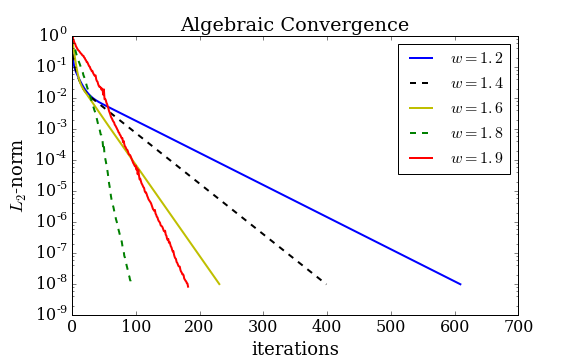
\includegraphics[width=0.5\textwidth]{algb_conv_c1_g1_w1_omega}\label{Algebraic Convergence}
\caption{Convergence of the SOR method for case 1 with a frequency of n=1. (Grid is 25 by 25) }
\end{figure}
%%%%%%%%%%%%%%%%%%%%%%%%%%%%%%%%%%%%%%%%%%

\noindent If we solve the same problem using a 100 by 100 grid instead of a 25 by 25 grid, we see that the solution requires more iterations, but more importantly, the overall error is reduced (from about 0.00528 to 0.00033). Additionally we see that $\omega = 1.9$ is more desirable in this case.

%%%%%%%%%%%%%%%%%%%%%%%%%%%%%%%%%%%%%%%
\begin{figure}[H]
\centering
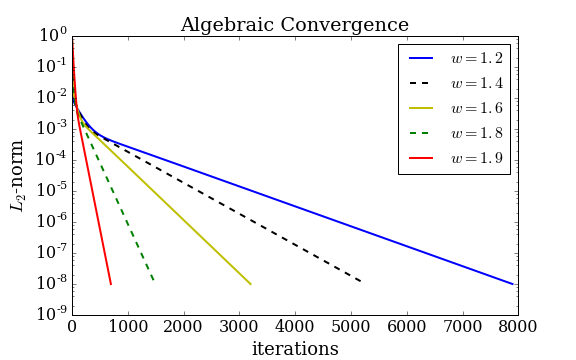
\includegraphics[width=0.5\textwidth]{algb_conv_c1_g3_w1_omega}\label{Algebraic Convergence}
\caption{Convergence of the SOR method for case 1 with a frequency of n=1. (Grid is 100 by 100)}
\end{figure}
%%%%%%%%%%%%%%%%%%%%%%%%%%%%%%%%%%%%%%%%%%

\noindent We should make sure that by improving the convergence cycles, we are not also increasing the error. Ideally we would want the error to remain the same if we only vary the relaxation parameter. In other words, for a given frequency, we want to increase convergence speed and also maintain accuracy. Continuing with our simple case of n=1, we see (Figure 8) that the error of the computed solution when compared to the analytical solution has not changed  as the relaxation parameter is varied(remains at about error = 0.0053 on a25 by 25 node grid), which is good news. Our error is stable. 

%%%%%%%%%%%%%%%%%%%%%%%%%%%%%%%%%%%%%%%
\begin{figure}[H]
\centering
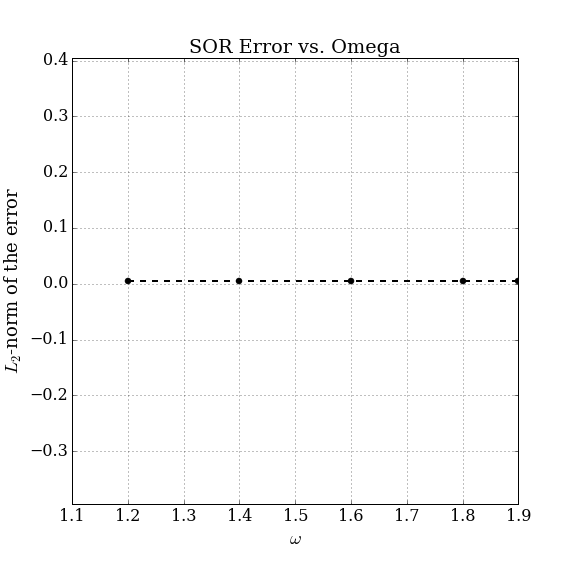
\includegraphics[width=0.5\textwidth]{err_an_c1_g1_w1_omega}\label{error}
\caption{Analytical error as a function of relaxation parameter for the SOR method}
\end{figure}
%%%%%%%%%%%%%%%%%%%%%%%%%%%%%%%%%%%%%%%%%%

\vspace{1em}

\noindent Now, we can proceed to look into another outstanding issue: \\

\vspace{0.5em}

\noindent $\textit{What is the impact of frequency on the requirements for grid resolution and convergence of the methods}?$ 

\vspace{1em}

\noindent To better understand, we can examine solutions for a  range of frequencies.  Generally, we can also choose a range of frequencies for each grid size by the following relationship:

\vspace{1 em}

\begin{equation}
1 \leq n_{frequency} \leq \frac{(min(n_{x},n_{y}))}{2} \nonumber
\end{equation}

\vspace{1em}

\noindent In order to keep the computational resources at a minimum, let's look at the lower end those frequencies. We will proceed with the following values:

\begin{equation}
f = [1.0, 2.0, 4.0, 8.0, 12.0] \nonumber
\end{equation}

\vspace{1em}

\noindent Let's solve these frequencies on our 25 by 25 grid first. Figure (9) tells us that if we increase the frequency of the source term and solve on a single grid, the error of the solution (defined as the  l2 norm of analytical vs computed solutions) then our error will also increase. This means that if we wish to solve the Poisson equation with source terms with high frequencies, we better make sure that we refine the grid to keep the error acceptably low. In the case shown in figure (9) the error went from 0.0053 at a frequency of 1, to an error of 1.28 at a frequency of 12 - that's a huge increase of more than two-hundred-fold!

%%%%%%%%%%%%%%%%%%%%%%%%%%%%%%%%%%%%%%%
\begin{figure}[H]
\centering
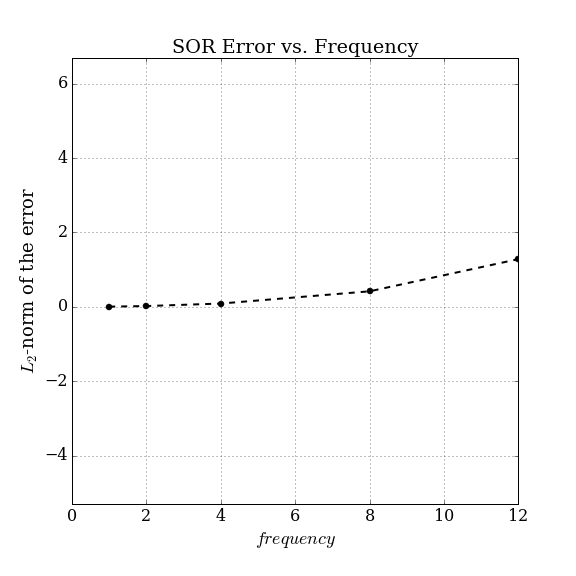
\includegraphics[width=0.4\textwidth]{err_an_c1_g1_nfreq}\label{Algebraic Convergence}
\caption{Error as a function of frequency }
\end{figure}
%%%%%%%%%%%%%%%%%%%%%%%%%%%%%%%%%%%%%%%%%%

\vspace{1em}

\noindent Now let's say we wanted to solve this case with a source term frequency of $n_f= 8.0$ and $n_f = 12.0$. The objective here is to refine the grid such that we keep the error down. Figure (10) shows that the grid was refined from a 25 by 25 grid, with the final grid being 200 by 200 nodes. The error was reduced from 0.42 to 0.0053.

%%%%%%%%%%%%%%%%%%%%%%%%%%%%%%%%%%%%%%%
\begin{figure}[H]
\centering
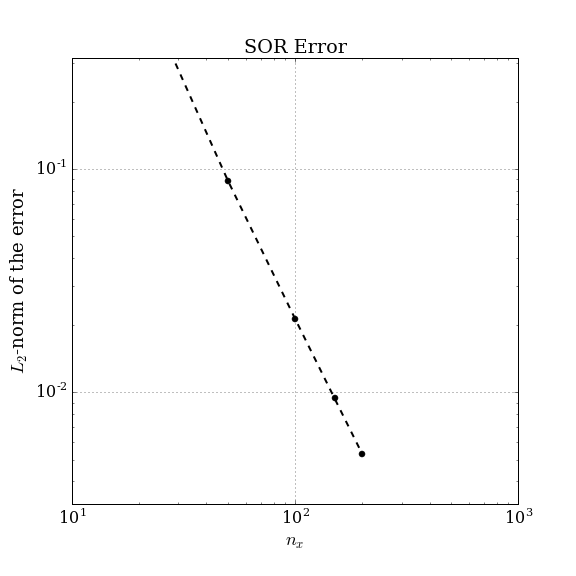
\includegraphics[width=0.4\textwidth]{errsor_c1_w4_nfreq}\label{Algebraic Convergence}
\caption{Error is reduced as the grid is refined for a frequency of 8.0}
\end{figure}
%%%%%%%%%%%%%%%%%%%%%%%%%%%%%%%%%%%%%%%%%%

\vspace{1em}

\noindent When we perform a similar analysis for a frequency of 12, we see that a grid of 25 by 25 nodes yields an l2 norm of the error of 1.28. When the grid is refined to 200 by 200 nodes, the error is reduced to 0.012. So, in order to reduce the error to levels comparable to the previous case, we must further refine the grid. Figure (11) shows the reduction in error due to grid refinement for a source term with a frequency of 12.

%%%%%%%%%%%%%%%%%%%%%%%%%%%%%%%%%%%%%%%
\begin{figure}[H]
\centering
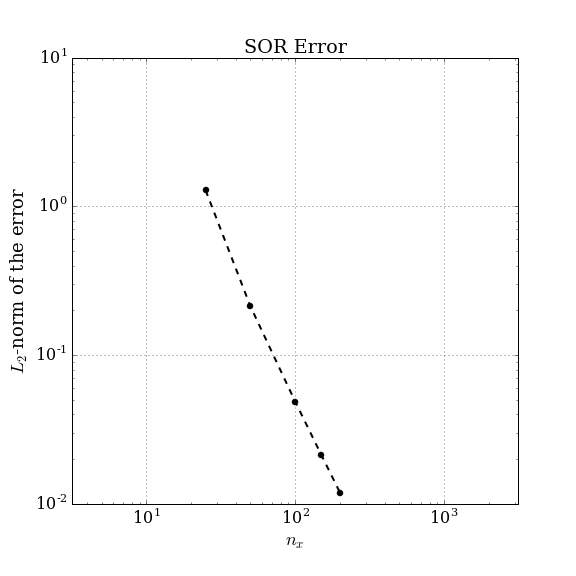
\includegraphics[width=0.4\textwidth]{errsor_c1_w5_nfreq}\label{Algebraic Convergence}
\caption{Error is reduced as the grid is refined for a frequency of 12.0}
\end{figure}
%%%%%%%%%%%%%%%%%%%%%%%%%%%%%%%%%%%%%%%%%%

\vspace{1em}

\subsection{Case 2: Homogeneous Neumann Boundary Conditions}

\noindent Similar to Case 1, we will analyze the computed solution by performing error analyses. We will, again, look at the simplest case: the solution for a frequency of $n = 1$. The number of grid points in x and y directions are both 25  nodes. The maximum and minimum values for the different methods are all within 99.9 percent of the analytical values. Additionally, figure (12) clearly shows the advantage of using the SOR method. It took the SOR method ($\omega = 1.9$) about 6 times less number of iterations to converge compared to the Jacobi method, and about 3 times less iterations than the Gauss-Sidel method.

%%%%%%%%%%%%%%%%%%%%%%%%%%%%%%%%%%%%%%%
\begin{figure}[H]
\centering
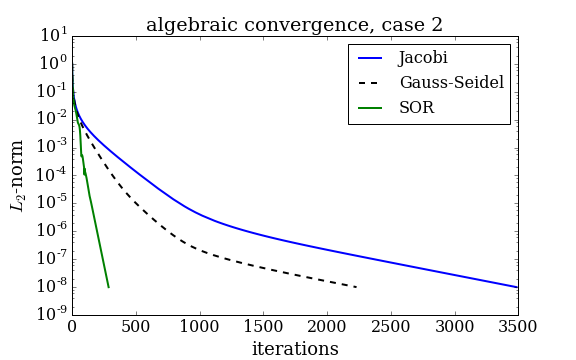
\includegraphics[width=0.7\textwidth]{algb_conv_c2_g1_w1}\label{Algebraic Convergence}
\caption{Convergence of the iterative methods for case 2 with a frequency of n=1. }
\end{figure}
%%%%%%%%%%%%%%%%%%%%%%%%%%%%%%%%%%%%%%%

\vspace{1em}

\noindent Figure (13) shows the 3- and 2-D graphs of the analytical and computed function.

%%%%%%%%%%%%%%%%%%%%%%%%%%%%%%%%%%%%%%%
\begin{figure}[H]
\centering
\subfigure[]{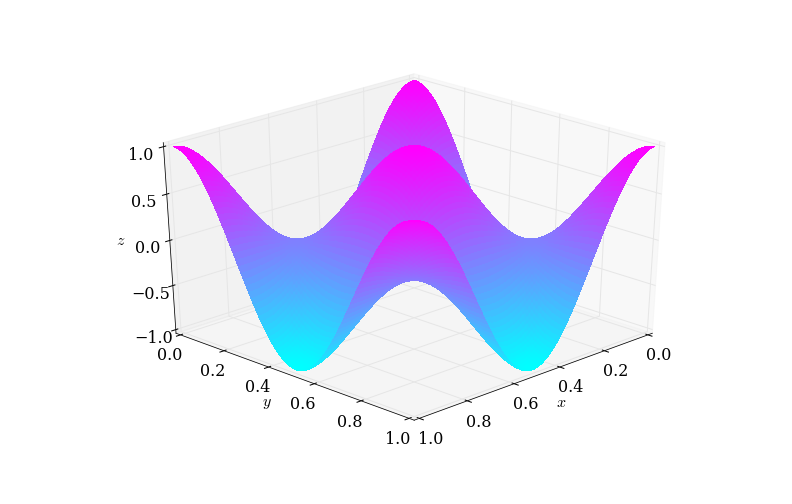
\includegraphics[width=0.4\textwidth]{p_an2_3d}\label{analytical function 3D}}
\subfigure[]{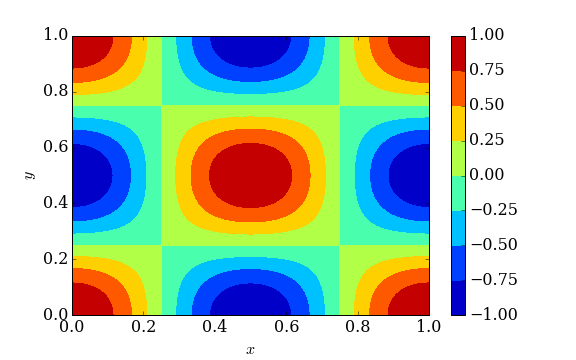
\includegraphics[width=0.4\textwidth]{p_an2_2d}\label{analytical function 2D}}
%\hspace{1em}
\subfigure[]{\includegraphics[width=0.4\textwidth]{J_3D_case2}\label{Jacobi 3D}}
\subfigure[]{\includegraphics[width=0.4\textwidth]{J_2D_case2}\label{Jacobi 2D}}
%\hspace{1em}
\subfigure[]{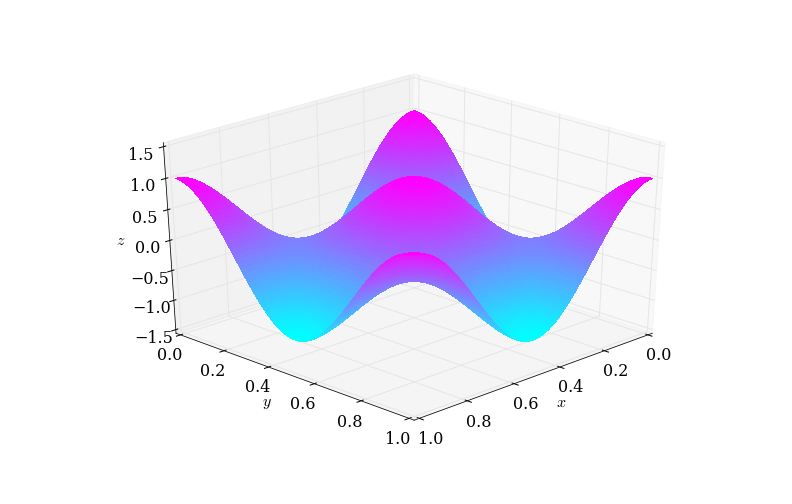
\includegraphics[width=0.4\textwidth]{pGS3dc2}\label{GS 3D}}
\subfigure[]{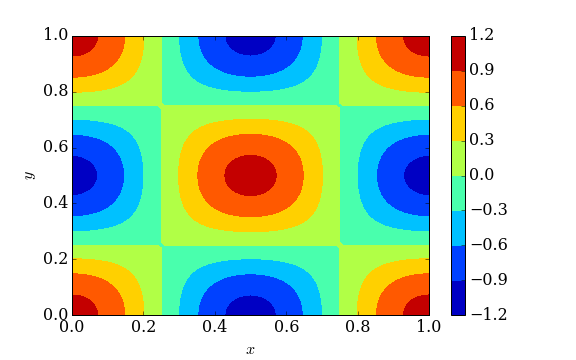
\includegraphics[width=0.4\textwidth]{pGS2dc2}\label{GS 2D}}
%\hspace{1em}
\subfigure[]{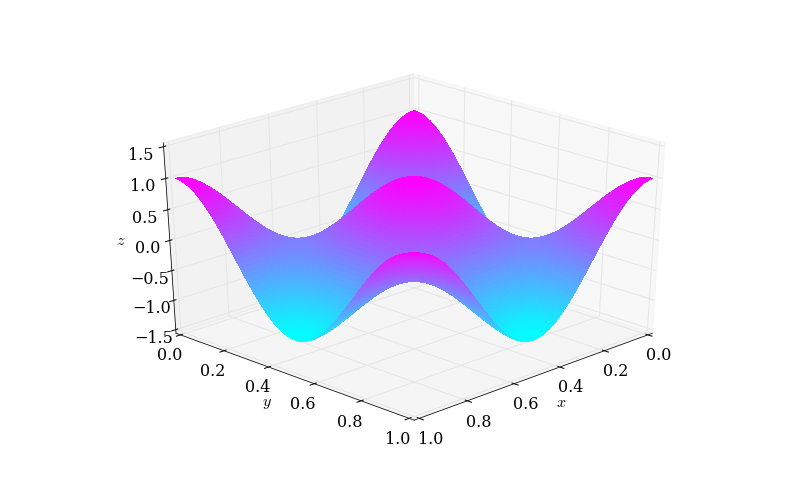
\includegraphics[width=0.4\textwidth]{pSOR3dc2}\label{SOR 3D}}
\subfigure[]{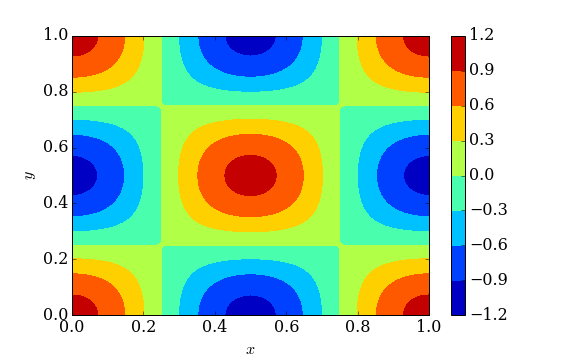
\includegraphics[width=0.4\textwidth]{pSOR2dc2}\label{SOR 2D}}
\caption{Visual comparison of analytical and computed solutions. (a-b) analytical solution, (b-c) Jacobi, (d-e) Gauss-Sidel, (f-g) SOR }
\end{figure}
%%%%%%%%%%%%%%%%%%%%%%%%%%%%%%%%%%%%%%%%%%

\noindent Now let's perform a grid refinement on the solution using the same array of nodes as part 1. Figure (14) shows that the error is reduced as nodes are increased and the rate of error decrease is consistent with our second-order discretization scheme.

%%%%%%%%%%%%%%%%%%%%%%%%%%%%%%%%%%%%%%%
\begin{figure}[H]
\centering
\subfigure[]{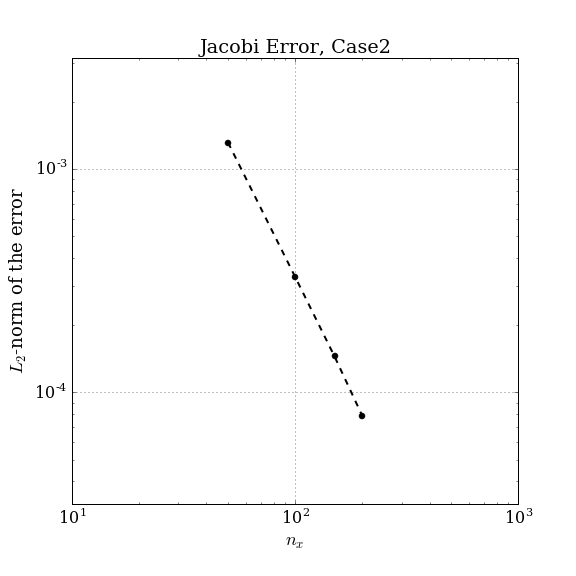
\includegraphics[width=0.5\textwidth]{errj_c2_g1_w1}\label{jacobi error 1}}
\subfigure[]{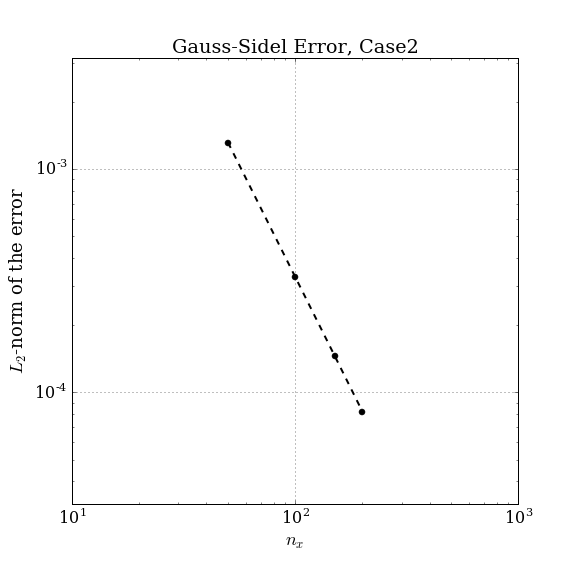
\includegraphics[width=0.5\textwidth]{errgs_c2_g1_w1}\label{gs error}}
\subfigure[]{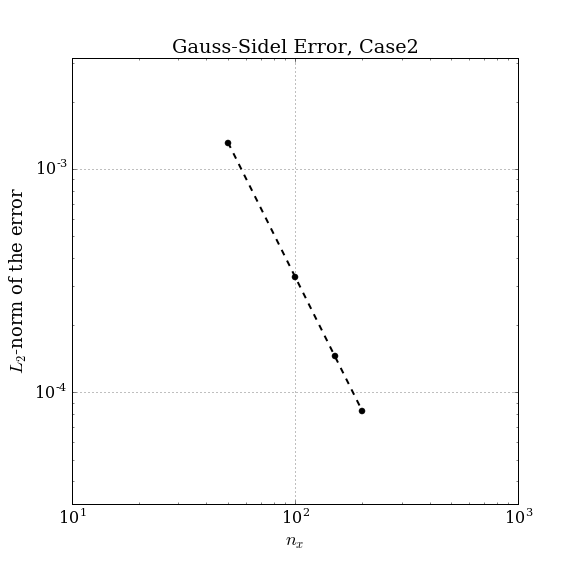
\includegraphics[width=0.5\textwidth]{errsor_c2_g1_w1}\label{sor error}}
\caption{Grid Refinement}
\end{figure}
%%%%%%%%%%%%%%%%%%%%%%%%%%%%%%%%%%%%%%%%%%

\vspace{1em}

\noindent Now let's look at how the SOR method converged using different relaxation parameters. Figure (15) shows that for the case of the 25 by 25 grid with a frequency of one, a relaxation parameter of 1.8 was optimal.

%%%%%%%%%%%%%%%%%%%%%%%%%%%%%%%%%%%%%%%
\begin{figure}[H]
\centering
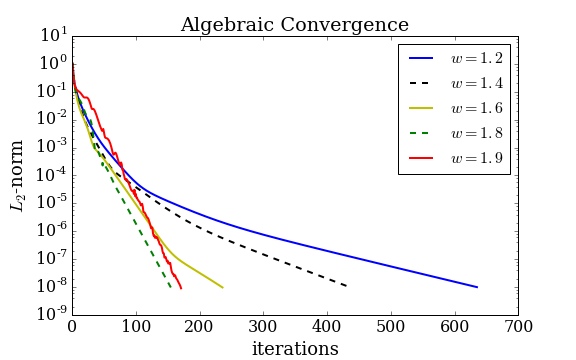
\includegraphics[width=0.5\textwidth]{algb_conv_c2_g1_w1_omega}\label{Algebraic Convergence}
\caption{Convergence of the SOR method for case 2 with a frequency of n=1. (Grid is 25 by 25) }
\end{figure}
%%%%%%%%%%%%%%%%%%%%%%%%%%%%%%%%%%%%%%%

\noindent Similarly to case 1, if we solve the same problem using a 100 by 100 grid instead of a 25 by 25 grid, we see that the solution requires more iterations, but the overall error is reduced (from about 0.00528 to 0.00033). We also see that $\omega = 1.9$ is more desirable in this case.

%%%%%%%%%%%%%%%%%%%%%%%%%%%%%%%%%%%%%%%
\begin{figure}[H]
\centering
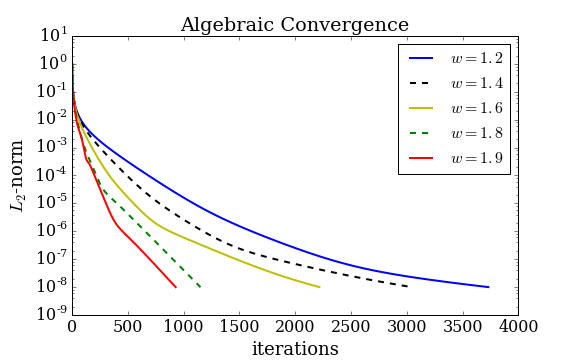
\includegraphics[width=0.5\textwidth]{algb_conv_c2_g3_w1_omega}\label{Algebraic Convergence}
\caption{Convergence of the SOR method for case 1 with a frequency of n=1. (Grid is 100 by 100) }
\end{figure}
%%%%%%%%%%%%%%%%%%%%%%%%%%%%%%%%%%%%%%%%%%


\vspace{1em}

\noindent We can also verify that the error remains constant given that omega is the only parameter allowed to change. This means that given that we keep our error low, there is substantial benefit in over-relaxation.

%%%%%%%%%%%%%%%%%%%%%%%%%%%%%%%%%%%%%%%
\begin{figure}[H]
\centering
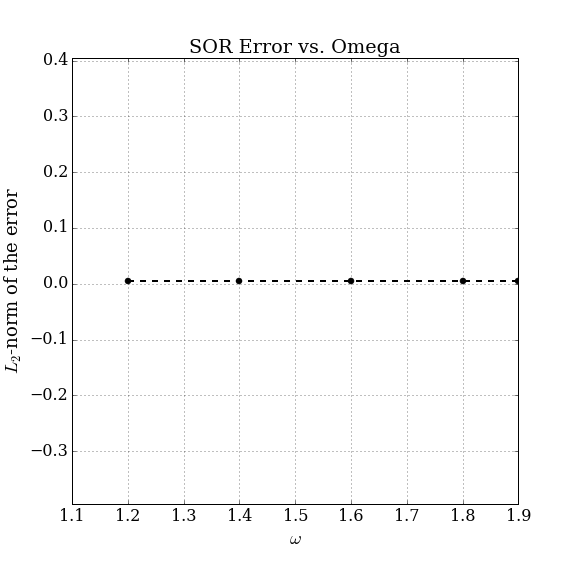
\includegraphics[width=0.5\textwidth]{err_an_c2_g1_w1_omega}\label{error}
\caption{Analytical error as a function of relaxation parameter for the SOR method}
\end{figure}
%%%%%%%%%%%%%%%%%%%%%%%%%%%%%%%%%%%%%%%%%%

\vspace{1em}

\noindent Similar to part 1, we solve for a range of frequencies on the same grid to examine how the error changes. Figure (18) shows that the error increases with higher frequencies. Again, we can say that if we wish to solve the Poisson equation for source terms with higher frequencies, we need to make sure that we employ a fine-enough mesh so that the error is reduced. In this chart, for a 25 by 25 grid, the error goes from 0.0053 (frequency=1) to 1.28 (frequency=12).

\vspace{1em}

\noindent By performing grid refinement fo the solutions of the Poisson equation with source terms that contain frequencies of 8 and 12, we see that the error decreases and the grid is refined. For the solution with a frequency of 8, we see that the error goes from 0.418 on a 25 by 25 grid to 0.00528 on a 200 by 200 grid. For a frequency of 12, we see that the error goes from 1.28 to 0.012 using the same grids. Again, this suggests that solutions with higher frequencies require more nodes to keep the error at the same level.

%%%%%%%%%%%%%%%%%%%%%%%%%%%%%%%%%%%%%%%
\begin{figure}[H]
\centering
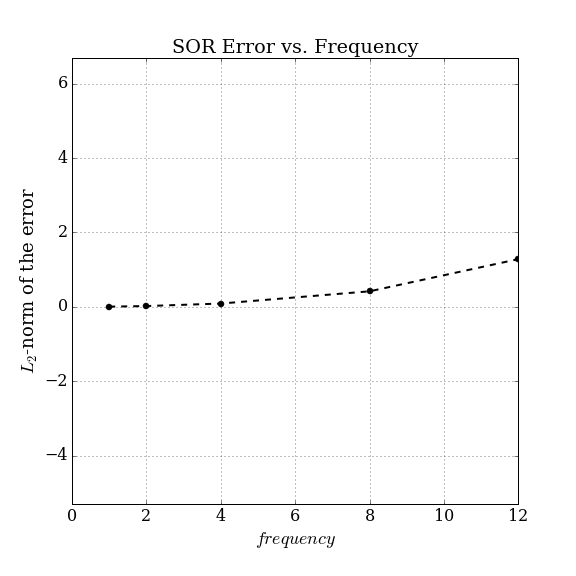
\includegraphics[width=0.4\textwidth]{err_an_c2_g1_nfreq}\label{Algebraic Convergence}
\caption{Error as a function of frequency }
\end{figure}
%%%%%%%%%%%%%%%%%%%%%%%%%%%%%%%%%%%%%%%%%%

%%%%%%%%%%%%%%%%%%%%%%%%%%%%%%%%%%%%%%%
\begin{figure}[H]
\centering
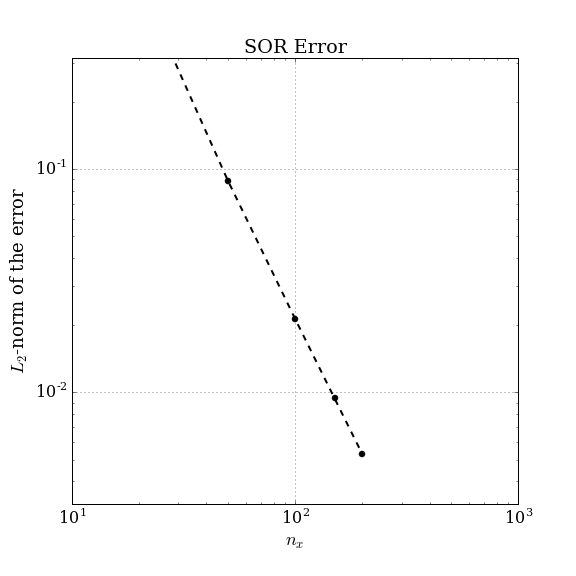
\includegraphics[width=0.4\textwidth]{errsor_c2_w4_nfreq}\label{Algebraic Convergence}
\caption{Error is reduced as the grid is refined for a frequency of 8.0}
\end{figure}
%%%%%%%%%%%%%%%%%%%%%%%%%%%%%%%%%%%%%%%%%%

%%%%%%%%%%%%%%%%%%%%%%%%%%%%%%%%%%%%%%%
\begin{figure}[H]
\centering
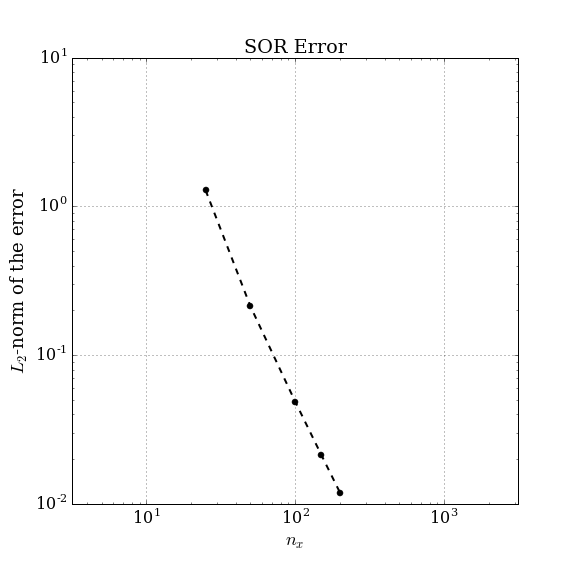
\includegraphics[width=0.4\textwidth]{errsor_c2_w5_nfreq}\label{Algebraic Convergence}
\caption{Error is reduced as the grid is refined for a frequency of 12.0}
\end{figure}
%%%%%%%%%%%%%%%%%%%%%%%%%%%%%%%%%%%%%%%%%%

\vspace{1em}

\section{Conclusions}

\noindent When we started this analysis, we wanted to be able to get a sense of how the relaxation parameter is affected by the frequency, grid size, and boundary conditions. After developing the code and looking at some results on the lower end of frequencies (in order to keep the grid size small due to computational restrictions), one of the most important aspects about developing an accurate solution is to make sure that the computed results closely resemble the analytical results. It is often the case that analytical results are not available, so experimental results can be helpful in validating the CFD models. If analytical solutions are available then ideally we are looking to keep the error as small as possible. It is in the context of maintaining a standard of accuracy that it is most productive to talk about what the optimal relaxation parameter is. Because, after all, if the error is large, it does not matter what relaxation parameter converges the fastest. 

\vspace{1em}

\noindent Looking at figures  6 and  7 for case 1, and figures  15 and 16 for case 2, I did notice that as we reduce the error, we increase the grid size, and it is in this range of very low errors that it is most optimal to use higher relaxation parameters. We don't necessarily want to increase the computational expense if not necessary, but if the errors are large enough it will be necessary to increase the grid. The results here show that an SOR method with a high relaxation parameter sort of "compensates" for the extra computations required to keep the error low.

\vspace{1em}

\noindent Another issue that I have not discussed at all, is the sensitivity of these iterative methods to initial conditions. For example, for case 1, I initiated the computational domain with random numbers from zero to one. For case 2, initializing the field in this way often led to very long computational times for convergence, or even to higher errors than expected. So for case 2, I had to initialize the flow field with all zero values, and this allowed the solver to converge faster with expected results.

\vspace{1em}

\noindent Finally, I have also derived and coded the model with a placement of nodes on cell boundaries (as opposed to cell centers) and the general trends discussed in this paper also hold for that model.

\end{document}
